\section{实验结果与分析}

本章节将介绍本实验的结果与分析,包括实验环境、实验结果、消融实验和实验分析。

\subsection{实验结果}

本实验对SimpleNet、SimpleNet with Dropout(并使用数据增强)、AlexNet 3种模型进行了训练和测试,得到了如图\ref{fig:results}所示的实验结果。如图所示,几种模型呈现出不同的效果,其中:

\begin{itemize}
    \item 如子图(a)(b)所示,SimpleNet在训练集上损失下降较快,但是在测试集上损失先下降后上升;同时SimpleNet在训练集上准确率很高,但是在测试集上准确率较低,出现了过拟合现象。
    \item 如子图(c)(d)所示,SimpleNet with Dropout(并使用数据增强)在训练集和测试集上的损失都不断下降,同时在训练集和测试集上的准确率都不断上升。虽然在测试集上的表现低于训练集,但是过拟合现象有所缓解。
    \item 如子图(e)(f)所示,AlexNet在训练集和测试集上的损失都不断下降,同时在训练集和测试集上的准确率都不断上升。AlexNet在测试集上的表现显著优于SimpleNet和SimpleNet with Dropout,表明AlexNet的泛化能力更强。
\end{itemize}

% pics目录下,simplenet_loss.png / simplenet_acc.png / dropout_loss.png / dropout_acc.png / alexnet_loss.png / alexnet_acc.png
% 每行放2张子图
\begin{figure}[H]
    \centering
    \subfloat[SimpleNet损失变化]{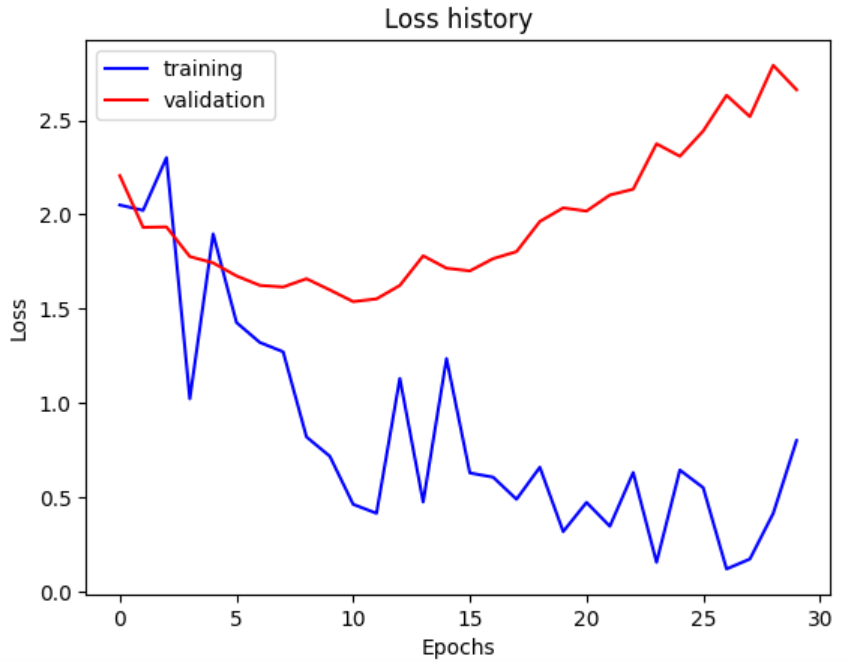
\includegraphics[width=0.4\textwidth]{pics/simplenet_loss.png}}
    \subfloat[SimpleNet准确率变化]{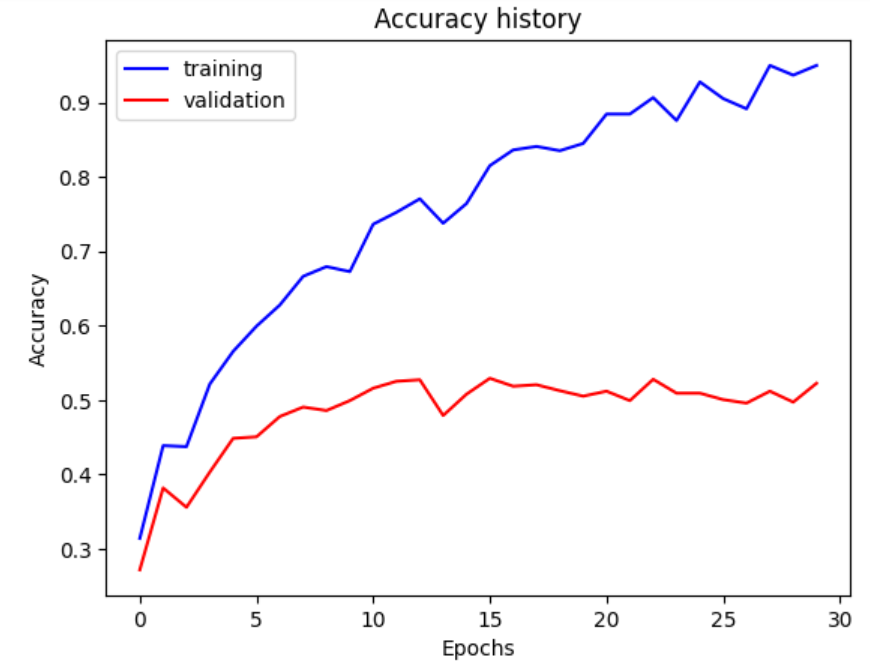
\includegraphics[width=0.4\textwidth]{pics/simplenet_acc.png}} \\
    \subfloat[SimpleNet with Dropout损失变化]{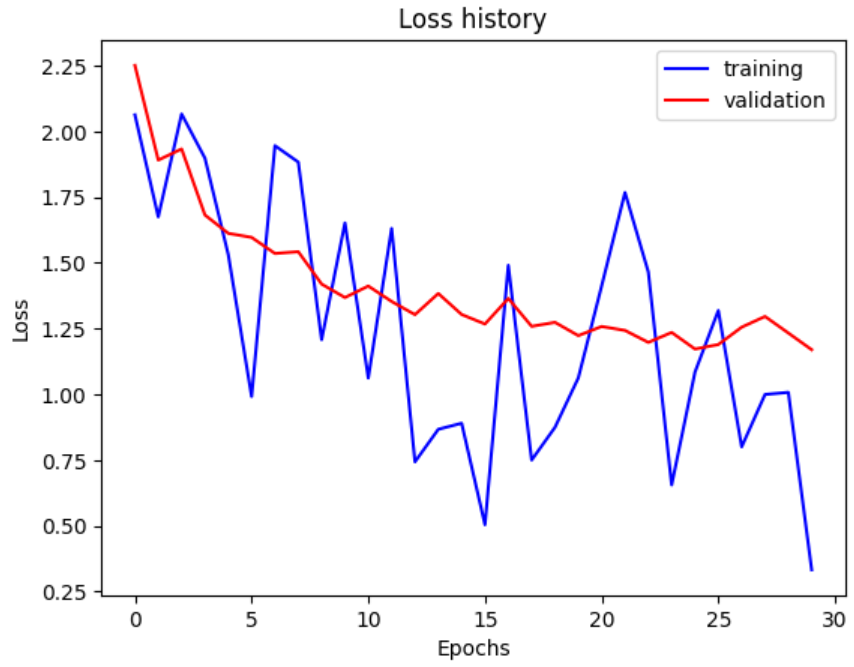
\includegraphics[width=0.4\textwidth]{pics/dropout_loss.png}}
    \subfloat[SimpleNet with Dropout准确率变化]{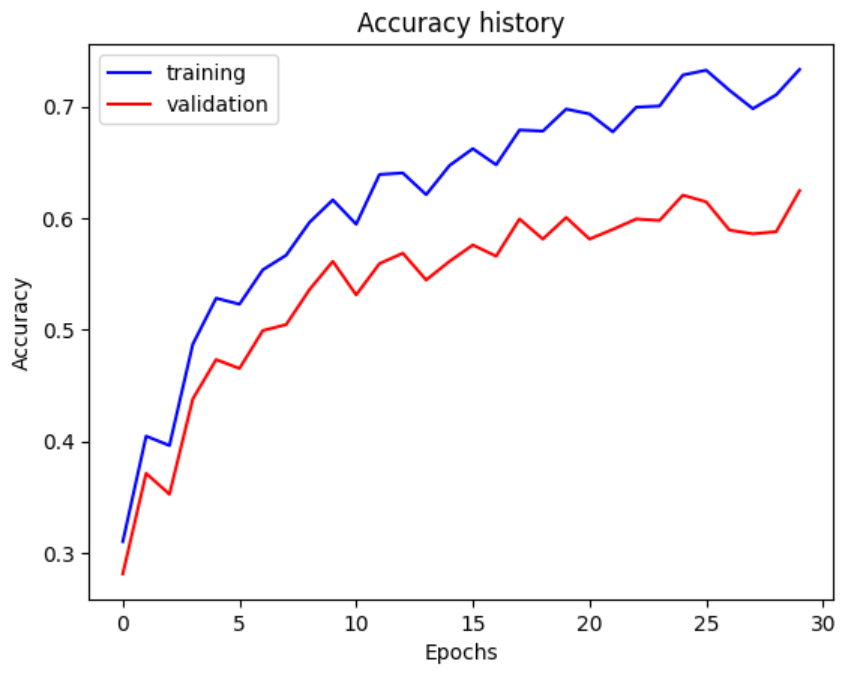
\includegraphics[width=0.4\textwidth]{pics/dropout_acc.png}} \\
    \subfloat[AlexNet损失变化]{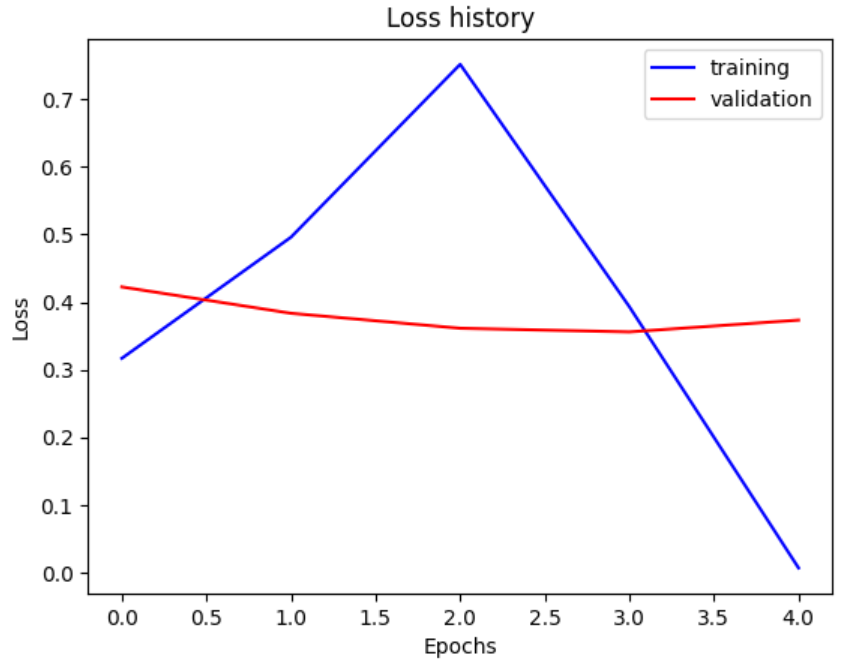
\includegraphics[width=0.4\textwidth]{pics/alexnet_loss.png}}
    \subfloat[AlexNet准确率变化]{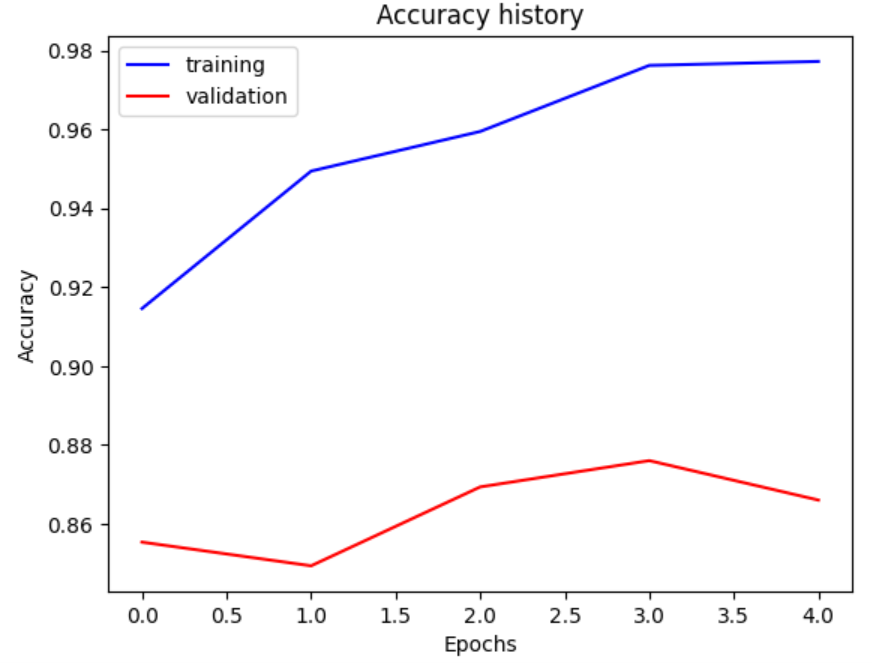
\includegraphics[width=0.4\textwidth]{pics/alexnet_acc.png}} \\
    \subfloat[Transformer损失变化]{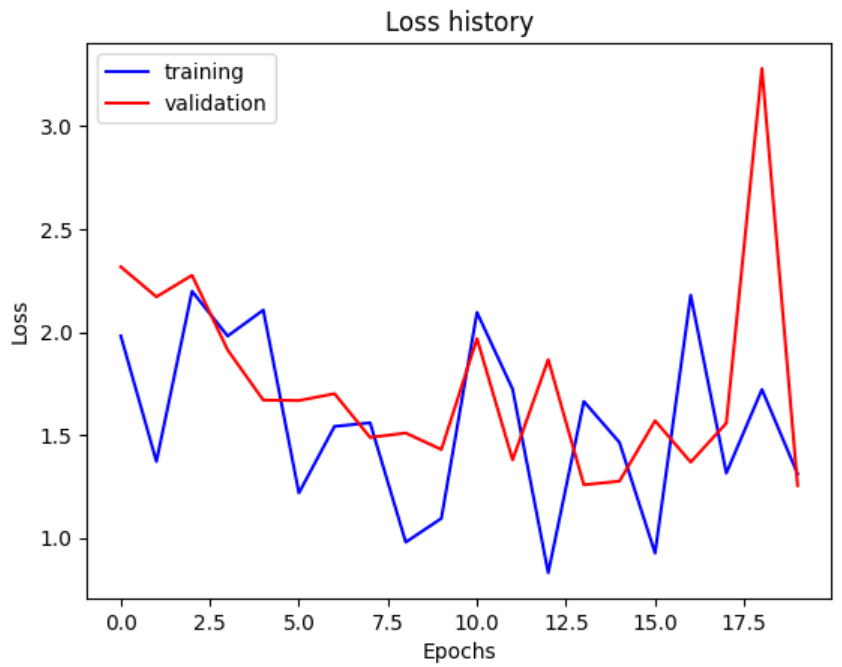
\includegraphics[width=0.4\textwidth]{pics/transformer_loss.png}}
    \subfloat[Transformer准确率变化]{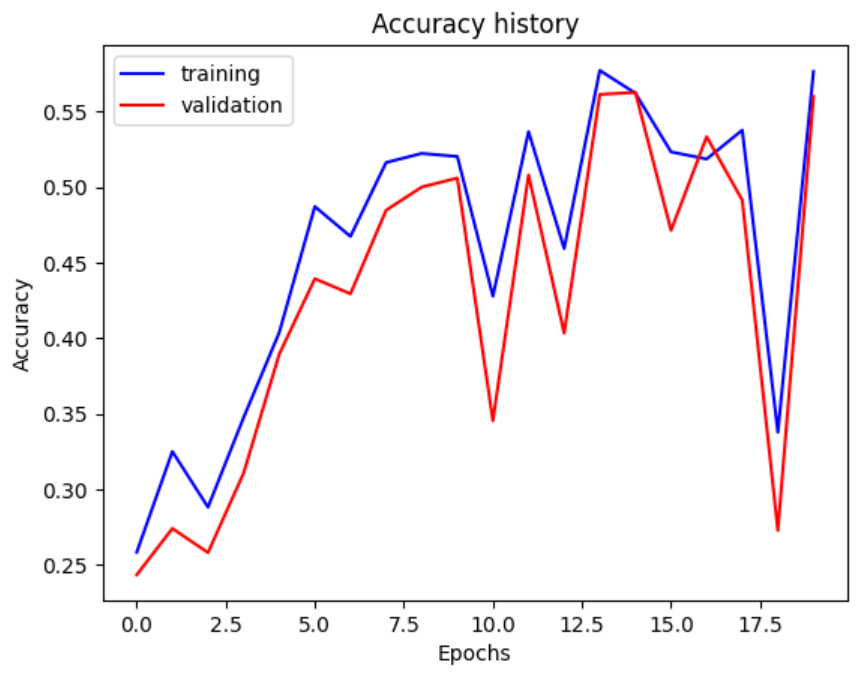
\includegraphics[width=0.4\textwidth]{pics/transformer_acc.png}}
    \caption{实验结果}
    \label{fig:results}
\end{figure}

各个模型的性能如表\ref{tab:performance}所示,可以看出:

\begin{itemize}
    \item SimpleNet在测试集上的准确率最低,且出现了严重的过拟合现象。
    \item SimpleNet with Dropout在测试集上的准确率次之,且过拟合现象有所缓解。
    \item AlexNet在测试集上的准确率相对来说很高,且泛化能力较强。
    \item 未经预训练的Transformer模型在测试集上的准确率较低。
    \item 经过预训练的Transformer模型在测试集上的准确率最高,且泛化能力最强。
\end{itemize}

\begin{table}[H]
    \centering
    \caption{各模型性能}
    \label{tab:performance}
    \begin{tabular}{c|c|c|c|c}
        \hline
        模型 & 数据增强 & 预训练 & 训练集准确率 & 测试集准确率 \\
        \hline
        SimpleNet & × & × & 0.950 & 0.523 \\
        SimpleNet with Dropout & √ & × & 0.733 & 0.625 \\
        AlexNet & √ & √ & 0.977 & 0.866 \\
        Transformer & √ & × & 0.576 & 0.560 \\
        Transformer & √ & √ & 0.898 & 0.875 \\
        \hline
    \end{tabular}
\end{table}

\subsection{消融实验}

为了探究Dropout模块,以及数据增强操作对模型性能的影响,本实验进行了消融实验。消融实验的结果如表\ref{tab:ablation}所示,可以看出:

\begin{itemize}
    \item 在SimpleNet基础上加入Dropout模块,测试集准确率上升,说明Dropout模块可以缓解过拟合现象。
    \item 在SimpleNet with Dropout基础上加入水平翻转操作,测试集准确率上升,说明水平翻转操作可以增加数据多样性。
    \item 在SimpleNet with Dropout基础上加入颜色抖动操作,测试集准确率上升,说明颜色抖动操作可以增加数据多样性。
    \item 在SimpleNet with Dropout基础上加入垂直翻转操作,测试集准确率下降,说明水平、垂直翻转操作不利于模型训练。
    \item 在SimpleNet with Dropout基础上加入随机裁剪操作,测试集准确率上升,说明随机裁剪操作可以增加数据多样性。
\end{itemize}

\begin{table}[H]
    \centering
    \caption{消融实验结果}
    \label{tab:ablation}
    \begin{tabular}{l|c|c}
        \hline
        模型 & 训练集准确率 & 测试集准确率 \\
        \hline
        SimpleNet & \textbf{0.950} & 0.523 \\
        + Dropout & 0.896 & 0.537 \\
        + Dropout、水平翻转 & 0.755 & 0.596 \\
        + Dropout、水平翻转、颜色抖动 & 0.783 & 0.603 \\
        + Dropout、水平、垂直翻转、颜色抖动 & 0.650 & 0.519 \\
        \textbf{+ Dropout、水平翻转、随机裁剪} & 0.733 & \textbf{0.625} \\
        \hline
    \end{tabular}
\end{table}

此外,本实验还探究了Dropout概率对模型性能的影响,如图\ref{fig:dropout}所示,测试集准确率随着Dropout概率的增加先上升后下降,在Dropout概率为0.5时达到最高值,之后快速下降。这说明Dropout取0.5时最佳,而Dropout概率过大会影响模型性能。

\begin{figure}
    \centering
    \begin{tikzpicture}
        \begin{axis}[
            xlabel=Dropout概率,
            ylabel=测试集准确率,
            xtick=data,
            xticklabels={0.0, 0.1, 0.2, 0.3, 0.4, 0.5, 0.6, 0.7, 0.8, 0.9},
            legend pos=north west,
            ymajorgrids=true,
            grid style=dashed,
        ]
        
        \addplot[color=blue, mark=*] coordinates {
            (0.0, 0.595)
            (0.1, 0.600)
            (0.2, 0.612)
            (0.3, 0.623)
            (0.4, 0.621)
            (0.5, 0.625)
            (0.6, 0.616)
            (0.7, 0.583)
            (0.8, 0.541)
            (0.9, 0.508)
        };
        
        \end{axis}
    \end{tikzpicture}
    \caption{Dropout概率与测试集准确率}
    \label{fig:dropout}
\end{figure}

\subsection{实验分析}

本实验通过对SimpleNet、SimpleNet with Dropout和AlexNet三种模型的训练和测试,探究了Dropout模块和数据增强操作对模型性能的影响。实验结果表明:

\begin{itemize}
    \item Dropout模块可以缓解过拟合现象,提高模型泛化能力。
    \item 数据增强操作可以增加数据多样性,提高模型性能。然而,不合理的数据增强操作可能会降低模型性能。例如,垂直翻转操作可能会产生不符合现实情况的图像,从而降低模型性能。
    \item AlexNet模型在测试集上的准确率更高,表明设计合理的网络结构可以提高模型性能。
    \item 未经预训练的Transformer模型在测试集上的准确率较低,而预训练之后的Transformer模型在测试集上的准确率最高,这是因为Transformer模型结构复杂、参数众多,需要大量数据进行训练,因此预训练可以极大提高模型性能。
\end{itemize}

训练集和测试集上的准确率可以用来评价模型的性能和泛化能力,当训练集上的准确率远高于测试集时,说明模型出现了过拟合现象。本实验中,SimpleNet模型出现了严重的过拟合现象,而Dropout和数据增强操作可以缓解这一现象。此外,预训练可以提高模型性能,增强模型泛化能力。